\documentclass[12pt]{report}
\usepackage[utf8]{inputenc}
\usepackage[russian]{babel}
%\usepackage[14pt]{extsizes}
\usepackage{listings}
\usepackage{graphicx}
\usepackage{amsmath,amsfonts,amssymb,amsthm,mathtools} 
\usepackage{pgfplots}
\usepackage{filecontents}
\usepackage{float}
\usepackage{indentfirst}
\usepackage{eucal}
\usepackage{enumitem}
%s\documentclass[openany]{book}
\frenchspacing

\usepackage{indentfirst} % Красная строка

\usetikzlibrary{datavisualization}
\usetikzlibrary{datavisualization.formats.functions}

\usepackage{amsmath}


% Для листинга кода:
\lstset{ %
	language=c,                 % выбор языка для подсветки (здесь это С)
	basicstyle=\small\sffamily, % размер и начертание шрифта для подсветки кода
	numbers=left,               % где поставить нумерацию строк (слева\справа)
	numberstyle=\tiny,           % размер шрифта для номеров строк
	stepnumber=1,                   % размер шага между двумя номерами строк
	numbersep=5pt,                % как далеко отстоят номера строк от подсвечиваемого кода
	showspaces=false,            % показывать или нет пробелы специальными отступами
	showstringspaces=false,      % показывать или нет пробелы в строках
	showtabs=false,             % показывать или нет табуляцию в строках
	frame=single,              % рисовать рамку вокруг кода
	tabsize=2,                 % размер табуляции по умолчанию равен 2 пробелам
	captionpos=t,              % позиция заголовка вверху [t] или внизу [b] 
	breaklines=true,           % автоматически переносить строки (да\нет)
	breakatwhitespace=false, % переносить строки только если есть пробел
	escapeinside={\#*}{*)}   % если нужно добавить комментарии в коде
}


\usepackage[left=2cm,right=2cm, top=2cm,bottom=2cm,bindingoffset=0cm]{geometry}
% Для измененных титулов глав:
\usepackage{titlesec, blindtext, color} % подключаем нужные пакеты
\definecolor{gray75}{gray}{0.25} % определяем цвет
\newcommand{\hsp}{\hspace{20pt}} % длина линии в 20pt
% titleformat определяет стиль
\titleformat{\chapter}[hang]{\Huge\bfseries}{\thechapter\hsp\textcolor{gray75}{|}\hsp}{0pt}{\Huge\bfseries}


% plot
\usepackage{pgfplots}
\usepackage{filecontents}
\usetikzlibrary{datavisualization}
\usetikzlibrary{datavisualization.formats.functions}

\begin{document}

\thispagestyle{empty}
\begin{titlepage}

\noindent \begin{minipage}{0.15\textwidth}
	
\includegraphics[width=\linewidth]{img/b_logo}
	\end{minipage}
	\noindent\begin{minipage}{0.9\textwidth}\centering
		\textbf{Министерство науки и высшего образования Российской Федерации}\\
		\textbf{Федеральное государственное бюджетное образовательное учреждение высшего образования}\\
		\textbf{~~~«Московский государственный технический университет имени Н.Э.~Баумана}\\
		\textbf{(национальный исследовательский университет)»}\\
		\textbf{(МГТУ им. Н.Э.~Баумана)}
	\end{minipage}
	
	\noindent\rule{18cm}{3pt}
	\newline\newline
	\noindent ФАКУЛЬТЕТ $\underline{\text{~~~~~~~~~~~~~~~~~~~«Информатика и системы управления»~~~~~~~~~~~~~~}}$ \newline\newline
	\noindent КАФЕДРА $\underline{\text{«Программное обеспечение ЭВМ и информационные технологии»}}$\newline\newline\newline\newline\newline
	
	\begin{center}
		\noindent\begin{minipage}{1.1\textwidth}\centering
			\Large\textbf{  Отчет по практике}\newline
			\textbf{Организация и проведение салона}
			\textbf{<<Шаг в будущее>>}\newline\newline
		\end{minipage}
	\end{center}
	
	

	\noindent\textbf{Студент} $\underline{\text{~~~~~~~~~~~~~~~~~~~~~~~~~~~~~~~~Сукочева А.~~~~~~~~~~~~~~~~~~~~~~~~~~~~~~~~~~~~~~~~~~~~~~~~~~~~~~~~~~~~~~}}$\newline\newline
	\noindent\textbf{Группа} $\underline{\text{~~~~~~~~~~~~~~~~~~~~~~~~~~~~~~~~~~~~ИУ7-63Б~~~~~~~~~~~~~~~~~~~~~~~~~~~~~~~~~~~~~~~~~~~~~~~~~~~~~~~~~~~~~~~~~}}$\newline\newline
	\noindent\textbf{Тип практики} $\underline{\text{~~~~~~~~~~~~~~~~~~~~~~~~~Производственная~~~~~~~~~~~~~~~~~~~~~~~~~~~~~~~~~~~~~~~~~~~~~~~~~~~~~}}$\newline\newline
	\noindent\textbf{Название предприятия} $\underline{\text{~~~~~~~~~~~~МГТУ им. Н. Э. Баумана, каф. ИУ7~~~~~~~~~~~~~~~~~~~~~~~~~~~}}$\newline\newline\newline\newline\newline\newline
	
	
	\noindent\begin{tabular}{lcc}
		Студент: ~~~~~~~~~~~~~~~~~~~~~~~~~~~~~~~~~~~~~~~~~~~~~~~~~~~~~~~~ & $\underline{\text{~~~~~~~~~~~~~~~~}}$ & $\underline{\text{~~Сукочева А.~~}}$     \\
																		  & \footnotesize подпись, дата           & \footnotesize Фамилия, И.О.              \\
		%& &  \\
		Преподаватель:                                                    & $\underline{\text{~~~~~~~~~~~~~~~~}}$ & $\underline{\text{~~~~Толпинская Н.Б.~~~}}$ \\
																		  & \footnotesize подпись, дата           & \footnotesize Фамилия, И. О.             \\
	\end{tabular}


\begin{center}
	\vfill
	Москва~---~\the\year
	~г.
\end{center}

\end{titlepage}

\tableofcontents

\chapter*{Введение}

Ежегодно кафедра ИУ7 проводит конкурс <<Шаг в будущее>> для абитуриентов.
В 2021 году данное мероприятие было проведено 15 марта. 

Целью практики являлась организация и проведения данного конкурса.

В рамках выполнения практики необходимо решить следующие задачи.

\begin{enumerate}
	\item Установить необходимое ПО.
	\item Составить схему рассадки участников и подготовить необходимые документы для проведения конкурса.
	\item Информирование абитуриентов, которые участвуют в конкурсе, о правилах проведения. 
	\item Изучение и оценка работ участников.
	\item Составление рецензий.
	% \item Подготовка аудитории к проведению конкурса.
	% \item Организация работы студенческого жюри.
	% \item Проверка работоспособности ПО после окончания конкурса.
	\item Вручение призов.
\end{enumerate}

\chapter{Основная часть}

\section{Установка необходимого ПО}

Для установки необходимого ПО нужно было знать, какое ПО нужно каждому участнику.
Поэтому до проведения конкурса был произведен обзвон каждого участника конкурса с целью 
уточнения необходимого им ПО. Для тех участников, которым необходим был стационарный компьютер
для презентации работы было установлено запрошенное ПО.
Список языков программирования, необходимых участникам:

\begin{itemize}
	\item Python3;
	\item C\#;
	\item .NET framework;
	\item Pascal ABC.NET;
	\item C++;
	\item Swift 5.
\end{itemize}

Также для проведения конкурса некоторым участникам необходим был интернет.
До проведения конкурса каждого участника спрашивали о необходимости в использовании интернета.
Если участнику нужен был интернет ему предлагалось авторизоваться через бауманскую сеть для получения интернета.

\section{Составление схемы рассадки участников и подготовление необходимых документов для проведения конкурса}

После получения информации от участников конкурса о том, нужен ли им стационарный компьютер или нет
была составлена рассадка, которая учитывала наличие собственного ноутбука. 
Были проверены стационарные компьютеры на работоспособность.

% Рассадка представлена на рис. \ref{ref:1}

% \begin{figure}[ht!]	
% 	\centering{
% 		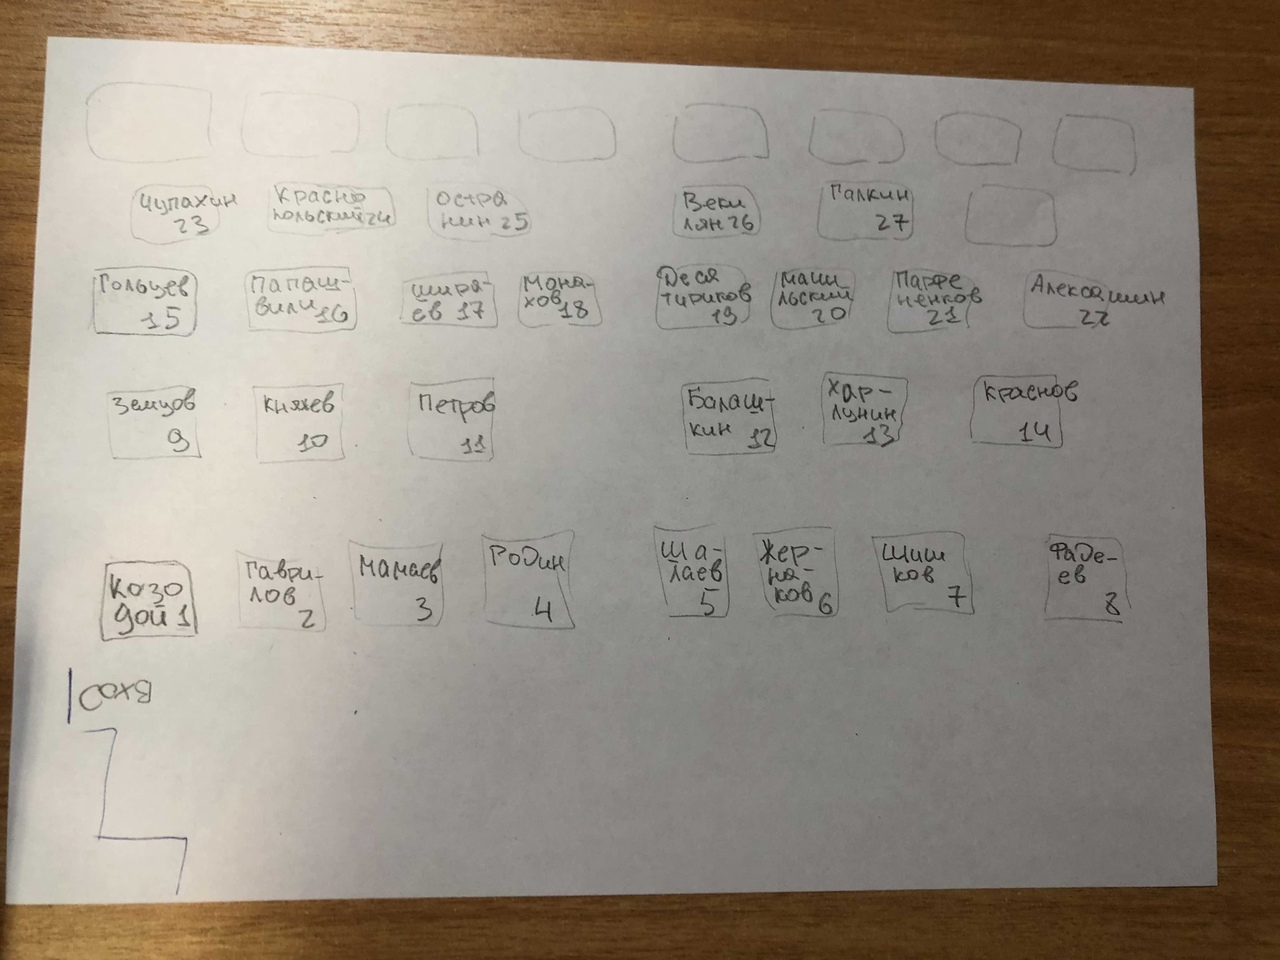
\includegraphics[width=0.9\textwidth]{img/img1.jpg}
% 		\caption{Рассадка участников конкурса}
% 		\label{ref:1}}
% \end{figure}

Для каждого участника конкурса был сделан бумажный указатель, идентифицирующий его проект, чтобы 
в дальнейшем каждый участник конкурса смог в точности знать свой стол. 

Также были распечатаны рецензии, которые заполнялись после проведения конкурса, 
листы с данными о каждом участнике, в котором они должны были расписываться за присутствие на конкурсе. 
Также были подготовлены именные бейджи для студенческого жюри и для членов экспертной комиссии. 

\section{Информирование абитуриентов, которые участвуют в конкурсе, о правилах проведения}

Предварительно нужно было информировать всех участников о дате проведения конкурса 
и о правилах. Организаторы имели список участников и их номера. 
Иногда номера были недоступны, тогда организаторы пытались найти участника в соц. сетях.

\chapter{Изучение работы участника}

\section{Сведения о участнике и его работе}

При проведении конкурса студенческое жюри просматривали и оценивали работы участников.
Проанализируем одну из работ.

Работа была сделана Козодоем Андреем Александровичем, учеником 11-Д класса школа №1580.
Тема рассматриваемой работы: <<Микросервисное API в операционной деятельности учебного заведения.
Мобильное приложение <<Мой МГТУ>>>> На рис. \ref{ref:2} показана работа одного из участника конкурса.

\begin{figure}[ht!]	
	\centering{
		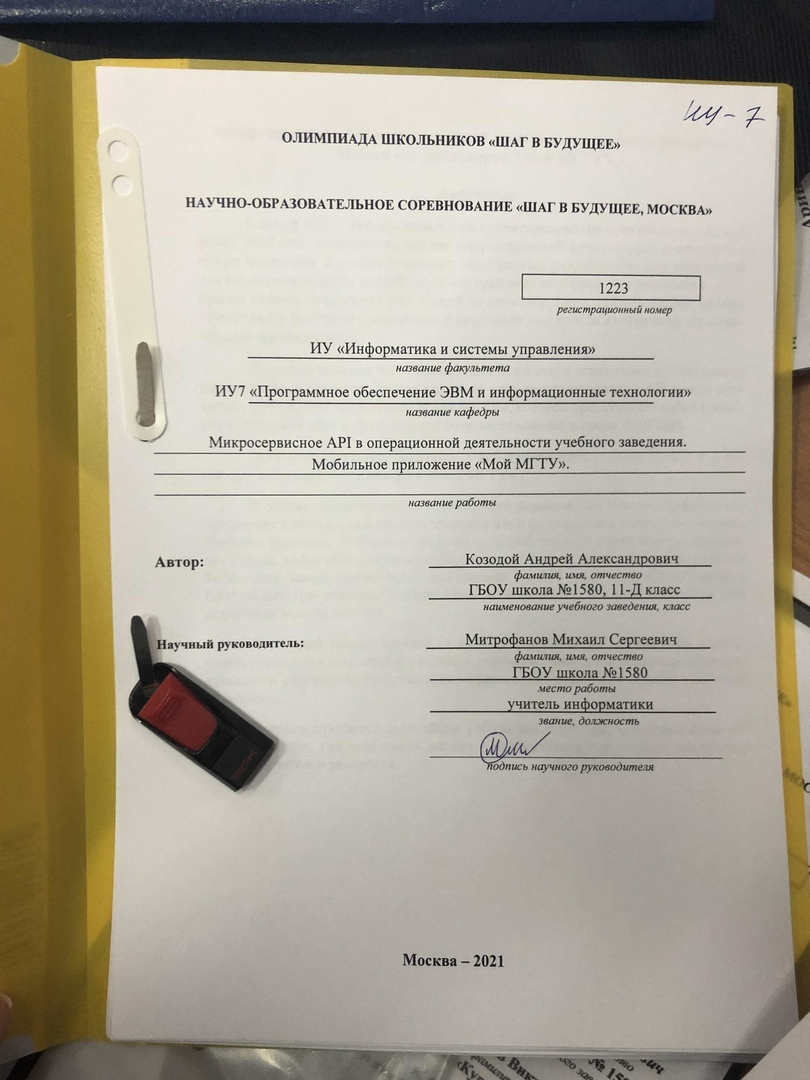
\includegraphics[width=0.9\textwidth]{img/img2.jpg}
		\caption{Работа одного из участника конкурса}
		\label{ref:2}}
\end{figure}

\section{Цель работы}

Работа данного участника была создана с целью внедрения в учебный процесс
собственных разрабатываемых технологий для автоматизации учебного процесса.
Она способствует внутреннему техническому развитию и обобщению знаний, внедрению этих знаний на практике.
Цели проекта рассматривают возможность быстрого расширения и адаптации под нужды
конкретной образовательной организации.

\section{Возможности предоставленного ПО}

В версии, которая была предоставлена на показ с помощью мобильного приложения, можно было
узнать расписание по классам, ученикам, учителям.
Новости и объявления образовательного учреждения представлены в 
формате социальных сетей <<историях>>.

Участник проекта предусматривал дальнейшую работу над проектом,
как дальнейшее исполнение плана, где глобальная миссия -- предоставить / дополнить платформу
высшего учебного заведения.

\section{Поставленные задачи}

Участник поставил перед собой задачу сделать динамическую и универсальную
платформу для образовательного учреждения, которую можно будет использовать
в высших учебных заведениях, школах, кружках. 

Участник провел опрос сверстников и проанализировал собранные материалы после чего 
выявил функциональность первой необходимости — это решение существующих
проблем с динамически изменяемым расписанием занятий и поиск друзей из других классов / групп.

\section{Оценка актуальности темы}

Участник заявил, что <<Согласно отзывам, действующие технологии, внедрённые в МГТУ, 
решают поставленные проблемы очень условно, где веб-сайт сервиса <<Электронный университет>>
представляет информацию недостаточно современно и удобно для ежедневного использования и поиска>>

Я считаю, что поставленная им задача неактуальна, т.к. в МГТУ имеется 
система контроля расписания и оценок. Данная система предоставляет почти все те возможности, 
которые разработал участник. 

\section{Архитектура приложения}

Для проекта была выбрана классическая системная архитектура,
с выделенными фронтэнда и бэкэнда рис. \ref{ref:3}.

\begin{figure}[ht!]	
	\centering{
		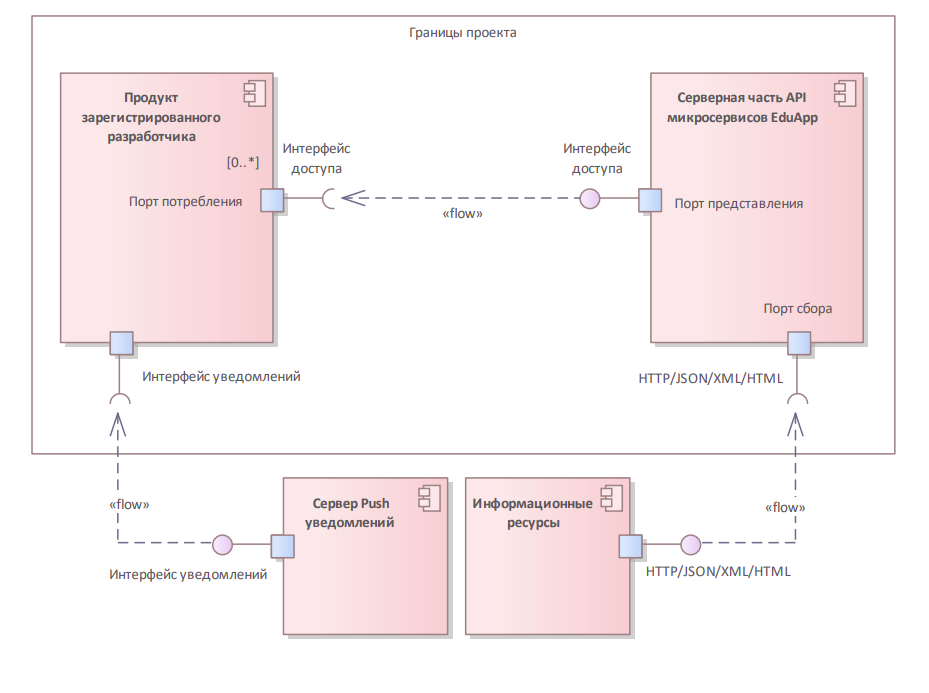
\includegraphics[width=0.9\textwidth]{img/img3.png}
		\caption{Системная архитектура}
		\label{ref:3}}
\end{figure}

Данная архитектура рекомендуется для мобильных приложений, работающих с данными, 
где в качестве фронтэнда выступает 
мобильное приложение <<Мой МГТУ>> непосредственно, а бэкэнд выполняет функции 
хранилища данных и исполняет скрипты автоматизации.

Стоит отметить, что участник конкурса использовал паттерн MVC (Model-View-Controller)
для организации приложения, что является несомненным плюсом в данной работе.

На рис. \ref{ref:4} показаны используемые в проекте ЯП и технологии.

\begin{figure}[ht!]	
	\centering{
		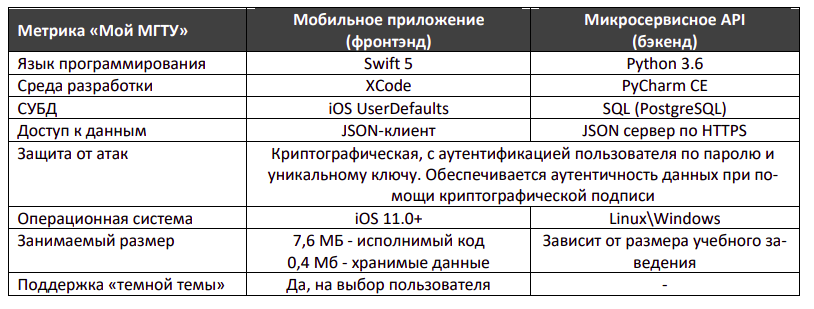
\includegraphics[width=0.9\textwidth]{img/img4.png}
		\caption{Фронтэнд и бэкэнд}
		\label{ref:4}}
\end{figure}

Для мобильного приложения <<Мой МГТУ>> экранные формы-наследники
UIViewController были созданы с помощью Storyboard - встроенного инструмента
среды разработки XCode. Данная функция помогает визуализировать связи 
контроллеров и внутренние графические элементы между собой риc. \ref{ref:5}

\begin{figure}[ht!]	
	\centering{
		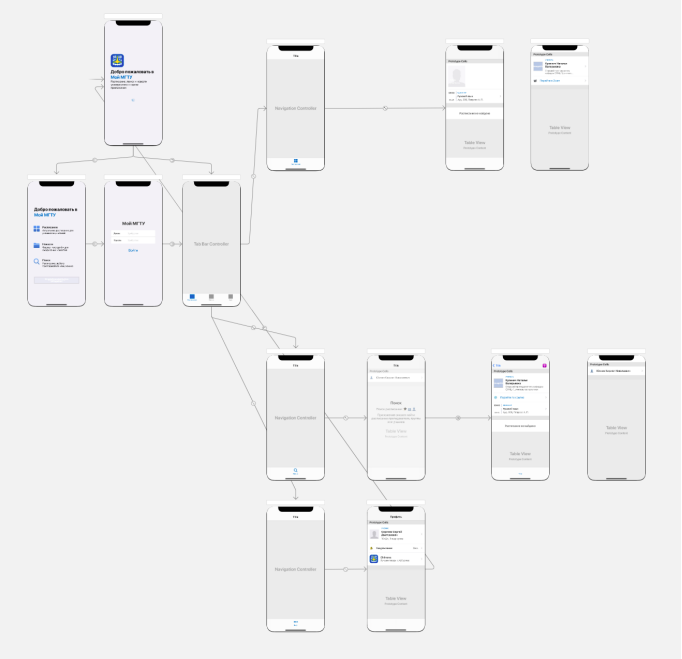
\includegraphics[width=0.9\textwidth]{img/img5.png}
		\caption{Модель экранных форм в виде Storyboard}
		\label{ref:5}}
\end{figure}

\section{Формирование базы данных}

Т.к. у участника конкурса во время разработки платформы
отсутствовал доступ к существующим информационным ресурсам 
<<Электронного университета>>, локальная задача формирования
базы данных была наиболее острой.
Участник принял решение о создании макетной базы данных,
основанной на имеющейся информации об учениках,
учителях и расписании в лицее 1580, с последующим переименованием 
существующих подгрупп в аналогичные по профилю в МГТУ.

Стоит отметить, что участник для получения списка учителей, должностей и групп с официального сайта
школы, предоставленного департаментом образования, разработал скрипт на языке программирования Python. 

\section{Преобразование собранных данных}

Т.к. сформированная участником база данных была основана для школы, он 
преобразовал школьные разделения по профилям по аналогии с разбиениями по кафедрам,
чтобы в дальнейшем легко преобразовать БД для МГТУ. На рис.  \ref{ref:6} - \ref{ref:7} представлено преобразование.  
Лицейским подгруппам были выданы случайные университетские группы
по данным кафедрам (курс и группа).

\begin{figure}[ht!]	
	\centering{
		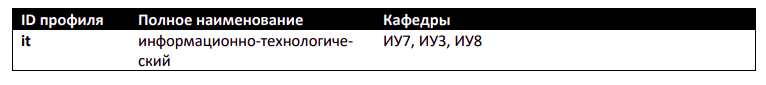
\includegraphics[width=0.9\textwidth]{img/img6.png}
		\caption{Преобразование собранных данных часть 1}
		\label{ref:6}}
\end{figure}

\begin{figure}[ht!]	
	\centering{
		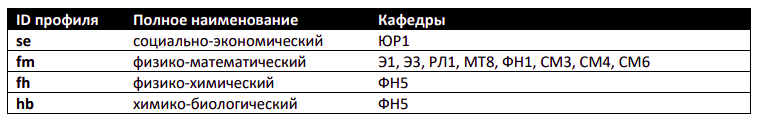
\includegraphics[width=0.9\textwidth]{img/img7.png}
		\caption{Преобразование собранных данных часть 2}
		\label{ref:7}}
\end{figure}

\section{Ролевые модели}

В предоставленном ПО были предусмотрены следующие модули пользователей:

% рис.  \ref{ref:8} 
% \begin{figure}[ht!]	
% 	\centering{
% 		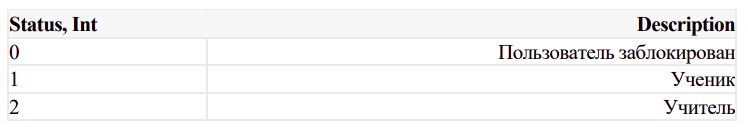
\includegraphics[width=0.9\textwidth]{img/img8.png}
% 		\caption{Модели пользователей}
% 		\label{ref:8}}
% \end{figure} 

\begin{itemize}
	\item 0 - пользователь заблокирован;
	\item 1 - ученик;
	\item 2 - учитель.
\end{itemize}

\section{Заключение}

Поставленные участником цели были достигнуты:

\begin{itemize}
	\item Разработана платформа учебного заведения. На базе данной платформы
	было разработано мобильное приложение <<Мой МГТУ>>, обладающее, согласно результатам опроса, функционалом первой необходимости: расписание, профили, подгруппы, поиск с фильтрами, уведомления о занятиях. Для
	разработчиков доступны библиотеки на языках программирования Swift и
	Python.
	\item Расширение платформы. Ученики-разработчики из лицея 1580 создали свои
	производные сервисы и продукты, которые в дальнейшем могут быть
	использованы в инфраструктуре МГТУ без дополнительных изменений
	в коде.
\end{itemize}

\chapter{Окончание конкурса}

\section{Вручение призов}

По окончанию проведения конкурса <<Шаг в будущее>>
было произведено голосование студенческого жюри и членов экспертной комиссии, 
по итогом которого было назначено 3 победителя. 

После чего всех участников пригласили на церемонию вручения призов, где трем победителям вручили призы.

\section{Составление рецензий}

Организаторы получили бланки для оценивания выступления и работы каждого участника.
Бланк состоит из двух частей -- оценки работы и резюме рецензента. 
В оценочной части необходимо поставить оценку от 0 до 4 по следующим критериям:

\begin{itemize}
	\item структура и оформление работы (качество оформления, грамотность содержания, ошибки, опечатки, выводы);
	\item логика изложения, оригинальность мышления, творческий подход;
	\item используемые методы (причины использования данных методов, эффективность, точность и простота методов);
	\item оригинальность тематики проекта, проверка текста научно-исследовательской на наличие заимствования из открытых
	источников в сети Интернет и других источников, актуальность тематики работы;
	\item научное и практическое значение работы;
\end{itemize}

На рис. \ref{ref:9} показан пример заполнения рецензии

\begin{figure}[ht!]	
	\centering{
		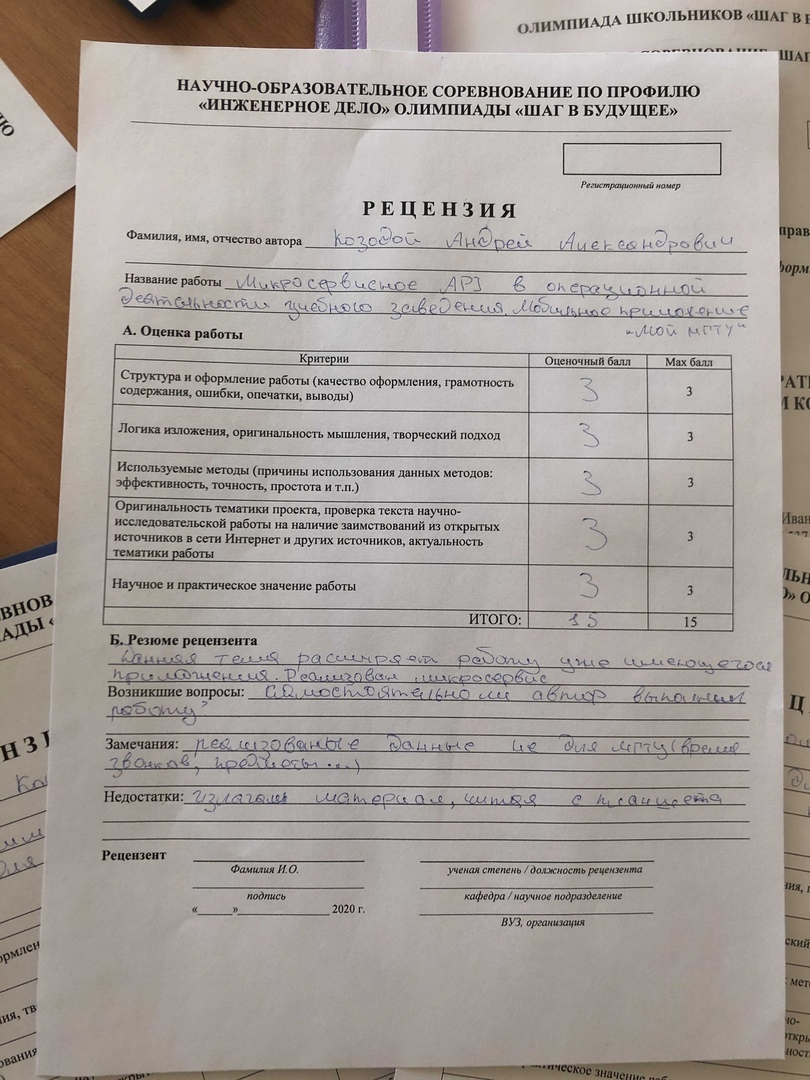
\includegraphics[width=0.9\textwidth]{img/img9.jpg}
		\caption{Пример заполнения рецензии}
		\label{ref:9}}
\end{figure} 

\chapter{Заключение}

Была пройдена практика по проведению программного салона <<Шаг в будущее>>.
Был организован конкурс, в результате которого были определены победители конкурса.
Руководство кафедры ИУ7 объявило устную благодарность организаторам салона.

Были выполнены следующие задачи.

\begin{enumerate}
	\item Установлено необходимое ПО.
	\item Составлена схема рассадки участников и подготовлены необходимые документы для проведения конкурса.
	\item Информированы абитуриенты, которые участвуют в конкурсе, о правилах проведения. 
	\item Изучена и оценена работа участника.
	\item Составлены рецензии.
	\item Вручены призы.
\end{enumerate}


Цель, поставленная во время прохождения практики, была достигнута. 

\end{document}
